\documentclass[italian]{unicam-thesis}

\title{Compilazione di un linguaggio funzionale in Java}

\university{Università degli Studi di Camerino}
\school{Scienze e Tecnologie}
\course{Laurea in Informatica (Classe L-31)}

\author{Massimo Pavoni}
\advisor{Prof. Luca Padovani}
\academicyear{2023/2024}
\matricola{124377}

\graphicspath{{resources/images/}}

\addbibresource{7-bibliography.bib}

\begin{document}

\pagenumbering{roman}

\maketitle

\tableofcontents

\begingroup
\let\cleardoublepage\relax
\let\clearpage\relax

\lstlistoflistings

\listoffigures

\listoftables

\endgroup

\cleardoublepage

\pagenumbering{arabic}

\chapter{\localized{Introduzione}{Introduction}}
\label{chap:1-introduction}

\section{Motivazione}
\label{sec:1-1-motivation}

I linguaggi di programmazione più diffusi non sempre possono essere classificati
solamente come procedurali, ad oggetti, logici o funzionali: soprattutto con la crescente adozione di linguaggi funzionali
nell'industria e il progresso della tecnologia per l'esecuzione di algoritmi paralleli, l'introduzione di nuove \textit{feature}
ispirate dalla programmazione funzionale è ben gradita dalla maggior parte degli sviluppatori.

\noindent Molti linguaggi moderni possono più opportunamente essere chiamati "ibridi" o "multi-paradigma",
in virtù della combinazione di diverse metodologie.


\texttt{Java} nello specifico, a partire dalla versione 8, è stato arricchito con nuovi strumenti e costrutti
che permettono di scrivere codice più conciso e dichiarativo: la domanda che ci si pone è quindi se sia possibile tradurre
un linguaggio funzionale in codice imperativo, sfruttando le nuove funzionalità così come la programmazione ad oggetti.

\section{Obiettivi}
\label{sec:1-2-objectives}

Il progetto di cui questo documento è relazione ha come obiettivo principale la pianificazione e costruzione
di un compilatore da codice sorgente funzionale a codice \texttt{Java}, con particolare attenzione alla semplicità
di traduzione data dalle varie \textit{feature} impiegate.


Il linguaggio dovrebbe essere sufficientemente espressivo da permettere la definizione di funzioni basilari
e l'uso della ricorsione; le performance di compilazione ed esecuzione non sono aspetti prioritari,
ma devono essere tali da consentire l'utilizzo pratico con fini educativi e dimostrativi. 

\section{Struttura della tesi}
\label{sec:1-3-thesis-structure}

Al fine di offrire un quadro completo dello studio effettuato e del progetto,
esplorando aspetti sia teorici che pratici, la tesi è suddivisa nei seguenti capitoli:
\begin{enumerate}
    \setcounter{enumi}{1}
    \item introduzione al paradigma funzionale e panoramica generale del linguaggio creato;
    \item nozioni sui sistemi di tipo per linguaggi funzionali, sistema adottato e inferenza;
    \item elenco delle caratteristiche di \texttt{Java} utili e primi esempi di traduzione;
    \item descrizione del software realizzato, dettagli d'implementazione e ulteriori esempi;
    \item conclusioni, risultati ottenuti, osservazioni finali e possibili sviluppi futuri.
\end{enumerate}

\chapter{Funx}
\label{chap:2-funx}

Questo capitolo descrive brevemente i linguaggi funzionali e le scelte effettuate
durante l'ideazione del linguaggio usato per il progetto: \textbf{Funx}.

\noindent Il nome nasce dall'unione dei due termini anglosassoni \textit{functional} e \textit{expression};
viene quindi pronunciato \textipa{["f2nIk"s]} in inglese, o comunque \textipa{[fàn\textperiodcentered èx]} in italiano.

\section{Linguaggi funzionali}
\label{sec:2-1-functional-languages}

Nonostante molti linguaggi non si possano confinare all'interno di un solo paradigma,
parlando di linguaggi di programmazione si fa spesso riferimento a due grandi categorie:
linguaggi imperativi e linguaggi dichiarativi.


I primi hanno caratteristiche direttamente legate al modello di calcolo di \textit{John Von Neumann},
a sua volta non dissimile dalla macchina di \textit{Alan Turing}.
Questi linguaggi sono usati per scrivere codice che segue una precisa sequenza di istruzioni,
la quale descrive più o meno esplicitamente i passi necessari per risolvere il problema affrontato.

\noindent Appartengono alla famiglia dei linguaggi di programmazione imperativi sia linguaggi procedurali come
\texttt{Fortran}, \texttt{Cobol} e \texttt{Zig}, sia i linguaggi orientati agli oggetti, tra cui \texttt{Kotlin}, \texttt{C\#} e \texttt{Ruby}.


I linguaggi dichiarativi, invece, sono fondamentali per lo scopo del progetto:
tali linguaggi sono generalmente di altissimo livello e permettono allo sviluppatore
di concentrarsi sull'obiettivo da raggiungere piuttosto che sui dettagli implementativi.

\noindent Fanno parte di questa categoria linguaggi di interrogazione come \texttt{SQL},
linguaggi logici come \texttt{Prolog} e soprattutto i linguaggi funzionali:
\texttt{Lisp}, \texttt{Clojure}, \texttt{Elixir}, \texttt{OCaml} e \texttt{Haskell} sono alcuni esempi.


Alla base di ogni linguaggio funzionale vi è il \textbf{lambda calcolo}%
\footnote{\citetitle{PostulatesFoundationLogic1}, \cite{PostulatesFoundationLogic1}
      e \citetitle{PostulatesFoundationLogic2} (Second paper), \cite{PostulatesFoundationLogic2}}:
un sistema formale definito dal matematico \textit{Alonzo Church} (supervisore di \textit{Alan Turing} durante il dottorato),
equivalente alla macchina di Turing, ma fondato sulle funzioni pure.

\newpage

\noindent La grammatica del lambda calcolo verrà presentata poco più avanti (sezione \ref{sec:2-3-syntax}),
ma le regole che ne governano il funzionamento e il modo in cui queste vengano utilizzate per ridurre
le espressioni ad una forma normale esulano dai fini di questo documento.

\noindent Rimane comunque rilevante elencare le principali qualità che un linguaggio funzionale
usualmente matura grazie al lambda calcolo:
\begin{itemize}
      \item \textbf{funzioni come entità di prima classe}: le funzioni possono essere passate come argomenti
            e restituite come risultato di altre funzioni;
      \item \textbf{immutabilità}: le variabili utilizzate sono immutabili;
      \item \textbf{purezza}: le funzioni sono libere da effetti collaterali
            (non modificano lo stato del programma) e restituiscono sempre lo stesso output per input identici;
      \item \textbf{ricorsione}: la ricorsione è il meccanismo più idiomatico per esprimere
            l'iterazione su una struttura dati.
\end{itemize}

\subsection{ML, Haskell e Funx}
\label{sec:2-2-ml-haskell-funx}

Nonostante le funzioni pure tipiche di un linguaggio funzionale siano un concetto molto attraente
dal punto di vista della correttezza della computazione, i vincoli così imposti possono risultare
stringenti a tal punto da rendere difficile, se non impossibile, la scrittura di programmi che
interagiscano con il mondo reale.


Per questo motivo, molti linguaggi funzionali permettono invece di utilizzare particolari funzioni
impure o di effettuare almeno operazioni di input/output. Inoltre, molti linguaggi prevalentemente
imperativi adottano ormai da tempo alcune caratteristiche tipiche dei linguaggi funzionali
(e.g. \texttt{Rust}, il linguaggio più amato%
\footnote{Stack Overflow Developer Survey 2023 (\url{https://survey.stackoverflow.co/2023}), \\
    \textit{Rust is the most admired language}}
dagli sviluppatori secondo i sondaggi di \textit{Stack Overflow},
eredita molto dal linguaggio con cui era scritto il suo primo compilatore, \texttt{OCaml}, ed è dotato quindi di
funzioni di prima classe, immutabilità di default, strutture dati algebriche, ecc.).


\texttt{ML} è un linguaggio funzionale sviluppato negli anni '70 presso l'Università di Edimburgo,
costituente la base per moltissimi dei linguaggi sviluppati in seguito.
\texttt{ML} permette effettivamente l'uso di funzioni impure, ma fra i suoi discendenti
vi è \texttt{Haskell}, uno dei pochi linguaggi invece completamente puri.

\noindent \texttt{Haskell} si avvale di un pattern di programmazione chiamato \textit{monadi}%
\footnote{\citetitle{Moggi-1991-ComputationMonads}, \cite{Moggi-1991-ComputationMonads}} per gestire
le operazioni di input/output e altre operazioni impure, mantenendo le funzioni pure.


Nell'ideare \textbf{Funx} l'ispirazione viene proprio da \texttt{Haskell}, ma è presente la possibilità
di dichiarare un'unica funzione impura (il cosiddetto \textit{main}) per permettere di visualizzare a schermo un risultato.
Il linguaggio non è quindi allo stesso livello di purezza di \texttt{Haskell}, e naturalmente non supporta
molte delle funzionalità più avanzate di quest'ultimo (come le \textit{classi di tipi} e il \textit{pattern matching}),
ma ne mutua altre comunque interessanti, tra cui l'uso di alcuni operatori infissi e il \textit{polimorfismo parametrico}.

\newpage

\section{Sintassi}
\label{sec:2-3-syntax}

La sintassi di \textbf{Funx} risulta molto simile a quella di \texttt{Haskell}, con poche differenze dovute
a tre principali motivi:
\begin{itemize}
    \item libera scelta di nomi e simboli per le parole chiave;
    \item necessità di successiva traduzione in \texttt{Java};
    \item difficoltà e scarso valore all'interno del progetto dell'implementazione di un parser dipendente dall'indentazione.
\end{itemize}

\noindent A prescindere da ciò, il cuore del linguaggio è lo stesso di ogni altro linguaggio derivato dal lambda calcolo:
la sua definizione si può agilmente comprendere visualizzando la grammatica del lambda calcolo e confrontandola con
quella (leggermente semplificata) di \textbf{Funx}, facendo attenzione alle regole aggiuntive.

\begin{figure}
    \vspace{4mm}
    \begin{bnf}
        $E$ : \small{Espressione} ::=
        | $x$ : \small{variabile}
        | $E_l\ E_r$ : \small{applicazione}
        | $\lambda x\ .\ E$ : \small{astrazione}
    \end{bnf}
    \caption{Grammatica del lambda calcolo}
    \label{fig:2-3-lambda-syntax}
    \vspace{4mm}
\end{figure}

\noindent Le tre regole in Figura~\ref{fig:2-3-lambda-syntax} indicano le tre componenti indispensabili
del lambda calcolo:
\begin{itemize}
    \item \textbf{variabile}: simbolo rappresentante un parametro;
    \item \textbf{applicazione}: applicazione di funzione ad un argomento (entrambi espressioni);
    \item \textbf{astrazione}: definizione di una funzione anonima, con un solo input $x$ (variabile vincolata)
          e un solo output $E$ (espressione); per definire funzioni con più
          parametri si debbono usare molteplici astrazioni annidate (tecnica detta \textit{currying}).
\end{itemize}

\newpage

\begin{figure}
    \begin{bnf}
        $M$ : \small{Modulo} ::=
        | $nome\ \cdot\ L$
        ;;
        $D$ : \small{Dichiarazione} ::=
        | $?(schema\ di\ tipo)\ \cdot\ id = E$ : \small{funzione}
        ;;
        $E$ : \small{Espressione} ::=
        | $c$ : \small{costante}
        | $x$ : \small{variabile}
        | $E_l\ E_r$ : \small{applicazione}
        | $\lambda x\ .\ E$ : \small{astrazione}
        | $L$ : \small{let}
        | $\textbf{if}\ E_c\ \textbf{then}\ E_t\ \textbf{else}\ E_e$ : \small{if}
        ;;
        $L$ : \small{Let} ::=
        | $\textbf{let}\ \cdot\ D\ (\cdot\ D)^*\ \cdot\ \textbf{in}\ E$
    \end{bnf}
    \caption{Grammatica di Funx}
    \label{fig:2-3-funx-syntax}
    \vspace{4mm}
\end{figure}

\noindent È facile constatare la presenza delle ulteriori produzioni per la definizione del modulo corrente
(informazione inclusa a prescindere dal fatto che il linguaggio ad ora non supporti l'importazione di moduli esterni
che non siano la libreria standard) e di funzioni con nome: lo \textit{schema di tipo} è un'informazione opzionale
relativa al tipo della funzione e di cui si parlerà più approfonditamente nella sezione~\ref{sec:3-3-system-fc}.

\noindent Per quanto riguarda invece le espressioni, vengono introdotte tre nuove regole:
\begin{itemize}
    \item \textbf{costante}: rappresenta un valore letterale, come un numero o una stringa;
    \item \textbf{let}: permette di avere dichiarazioni locali utilizzabili all'interno di un'espressione;
    \item \textbf{if}: la più classica istruzione condizionale controllata da un'espressione booleana.
\end{itemize}

\subsection{Zucchero sintattico}
\label{sec:2-4-syntactic-sugar}

Con lo scopo di rendere il codice più leggibile, conciso e semplice, \textbf{Funx} introduce
dello zucchero sintattico (del tutto simile a quello di \texttt{Haskell}).
In Tabella~\ref{tab:2-4-sugar} sono riportati l'indispensabile per evitare il parsing dell'indentazione,
le semplificazioni comuni utili all'arricchimento del lambda calcolo, e infine tutti gli operatori simbolici
supportati al momento (assieme alla notazione per indicarne associatività e precedenza).

\newpage

\begin{table}[H]
    \begin{center}
        \begin{tabularx}{\textwidth}{|P{15em}|X|}
            \hline
            \textbf{Zucchero}                & \textbf{Sostituzione}                                            \\
            \hline
            \texttt{$\backslash$x -> e}      & \texttt{$\lambda$x $\mathord{.}$ e}                              \\
            \hline
            \texttt{$\backslash$x y -> e}    & \texttt{$\lambda$x $\mathord{.}$ $\lambda$y $\mathord{.}$ e}     \\
            \hline
            \texttt{f x y = e}               & \texttt{f = $\lambda$x $\mathord{.}$ $\lambda$y $\mathord{.}$ e} \\
            \hline
            \texttt{let}                     &                                                                  \\
            \texttt{f1 = e1}                 & \texttt{let f1 = e1 $\cdot$ f2 = e2 in e3}                       \\
            \texttt{f2 = e2}                 &                                                                  \\
            \texttt{in e3}                   &                                                                  \\
            \hline
            \texttt{f3 = e3}                 &                                                                  \\
            \texttt{with}                    &                                                                  \\
            \texttt{f1 = e1}                 & \texttt{f3 = let f1 = e1 $\cdot$ f2 = e2 in e3}                  \\
            \texttt{f2 = e2}                 &                                                                  \\
            \texttt{out}                     &                                                                  \\
            \hline
            \texttt{main = e3}               &                                                                  \\
            \texttt{f1 = e1}                 & \texttt{main = let f1 = e1 $\cdot$ f2 = e2 in e3}                \\
            \texttt{f2 = e2}                 &                                                                  \\
            \hline
            \texttt{if b then e1 else e2 fi} & \texttt{if b then e1 else e2}                                    \\
            \hline
        \end{tabularx}
        % divide et impera because inconsistent tabbing is a thing
        \begin{tabularx}{\textwidth}{|P{7em}@{\quad}P{7em}|X|}
            \texttt{e1 $\mathord{.}$ e2} & \texttt{infixr 9} & \texttt{compose e1 e2}            \\
            \texttt{e1 / e2}             & \texttt{infixl 7} & \texttt{divide e1 e2}             \\
            \texttt{e1 \% e2}            & \texttt{infixl 7} & \texttt{modulo e1 e2}             \\
            \texttt{e1 * e2}             & \texttt{infixl 7} & \texttt{multiply e1 e2}           \\
            \texttt{e1 + e2}             & \texttt{infixl 6} & \texttt{add e1 e2}                \\
            \texttt{e1 - e2}             & \texttt{infixl 6} & \texttt{subtract e1 e2}           \\
            \texttt{e1 > e2}             & \texttt{infix 4}  & \texttt{greaterThan e1 e2}        \\
            \texttt{e1 >= e2}            & \texttt{infix 4}  & \texttt{greaterThanEquals e1 e2}  \\
            \texttt{e1 < e2}             & \texttt{infix 4}  & \texttt{lessThan e1 e2}           \\
            \texttt{e1 <= e2}            & \texttt{infix 4}  & \texttt{lessThanEquals e1 e2}     \\
            \texttt{e1 == e2}            & \texttt{infix 4}  & \texttt{equalsEquals e1 e2}       \\
            \texttt{e1 != e2}            & \texttt{infix 4}  & \texttt{notEquals e1 e2}          \\
            \texttt{!!e}                 & \texttt{prefix 4} & \texttt{not e}                    \\
            \texttt{e1 \&\& e2}          & \texttt{infixr 3} & \texttt{if e1 then e2 else False} \\
            \texttt{e1 || e2}            & \texttt{infixr 2} & \texttt{if e1 then True else e2}  \\
            \texttt{e1 \$ e2}            & \texttt{infixr 0} & \texttt{apply e1 e2}              \\
            \hline
        \end{tabularx}
    \end{center}
    \caption{Zucchero sintattico}
    \label{tab:2-4-sugar}
\end{table}

\newpage

\noindent Come già accennato, il Capitolo~\ref{chap:5-compiler} illustrerà come l'albero sintattico astratto (\textbf{AST})
di un programma viene ottenuto, annotato e tradotto in \texttt{Java}; la sezione~\ref{sec:4-2-ternary-operator}
esporrà invece il motivo della traduzione degli operatori booleani binari in if.

\noindent Alcuni esempi di funzioni sono presentati nel Codice~\ref{lst:2-4-example-funx};
seppur superflua, l'indentazione è inclusa per maggiore chiarezza.

\vspace{4mm}
\begin{lstlisting}[caption={Esempio di programma}, style=funxCode, label={lst:2-4-example-funx}]
main = factorial 20

factorial : Int @-> Int
factorial n = if n == 0 then 1 else n * factorial (n - 1) fi

even : Int @-> Bool
even = let
        even1 : Int @-> Bool
        even1 n = if n == 0 then True else odd (n - 1) fi

        odd : Int @-> Bool
        odd n = if n == 0 then False else even1 (n - 1) fi
    in even1

gcd : Int @-> Int @-> Int
gcd a b = if b == 0 then a else gcd b (a % b) fi

xor : Bool @-> Bool @-> Bool
xor a b = (a || b) && !!(a && b)
\end{lstlisting}

\subsection{Zucchero sintattico}
\label{sec:2-4-syntactic-sugar}

Con lo scopo di rendere il codice più leggibile, conciso e semplice, \textbf{Funx} introduce
dello zucchero sintattico (del tutto simile a quello di \texttt{Haskell}).
In Tabella~\ref{tab:2-4-sugar} sono riportati l'indispensabile per evitare il parsing dell'indentazione,
le semplificazioni comuni utili all'arricchimento del lambda calcolo, e infine tutti gli operatori simbolici
supportati al momento (assieme alla notazione per indicarne associatività e precedenza).

\newpage

\begin{table}[H]
    \begin{center}
        \begin{tabularx}{\textwidth}{|P{15em}|X|}
            \hline
            \textbf{Zucchero}                & \textbf{Sostituzione}                                            \\
            \hline
            \texttt{$\backslash$x -> e}      & \texttt{$\lambda$x $\mathord{.}$ e}                              \\
            \hline
            \texttt{$\backslash$x y -> e}    & \texttt{$\lambda$x $\mathord{.}$ $\lambda$y $\mathord{.}$ e}     \\
            \hline
            \texttt{f x y = e}               & \texttt{f = $\lambda$x $\mathord{.}$ $\lambda$y $\mathord{.}$ e} \\
            \hline
            \texttt{let}                     &                                                                  \\
            \texttt{f1 = e1}                 & \texttt{let f1 = e1 $\cdot$ f2 = e2 in e3}                       \\
            \texttt{f2 = e2}                 &                                                                  \\
            \texttt{in e3}                   &                                                                  \\
            \hline
            \texttt{f3 = e3}                 &                                                                  \\
            \texttt{with}                    &                                                                  \\
            \texttt{f1 = e1}                 & \texttt{f3 = let f1 = e1 $\cdot$ f2 = e2 in e3}                  \\
            \texttt{f2 = e2}                 &                                                                  \\
            \texttt{out}                     &                                                                  \\
            \hline
            \texttt{main = e3}               &                                                                  \\
            \texttt{f1 = e1}                 & \texttt{main = let f1 = e1 $\cdot$ f2 = e2 in e3}                \\
            \texttt{f2 = e2}                 &                                                                  \\
            \hline
            \texttt{if b then e1 else e2 fi} & \texttt{if b then e1 else e2}                                    \\
            \hline
        \end{tabularx}
        % divide et impera because inconsistent tabbing is a thing
        \begin{tabularx}{\textwidth}{|P{7em}@{\quad}P{7em}|X|}
            \texttt{e1 $\mathord{.}$ e2} & \texttt{infixr 9} & \texttt{compose e1 e2}            \\
            \texttt{e1 / e2}             & \texttt{infixl 7} & \texttt{divide e1 e2}             \\
            \texttt{e1 \% e2}            & \texttt{infixl 7} & \texttt{modulo e1 e2}             \\
            \texttt{e1 * e2}             & \texttt{infixl 7} & \texttt{multiply e1 e2}           \\
            \texttt{e1 + e2}             & \texttt{infixl 6} & \texttt{add e1 e2}                \\
            \texttt{e1 - e2}             & \texttt{infixl 6} & \texttt{subtract e1 e2}           \\
            \texttt{e1 > e2}             & \texttt{infix 4}  & \texttt{greaterThan e1 e2}        \\
            \texttt{e1 >= e2}            & \texttt{infix 4}  & \texttt{greaterThanEquals e1 e2}  \\
            \texttt{e1 < e2}             & \texttt{infix 4}  & \texttt{lessThan e1 e2}           \\
            \texttt{e1 <= e2}            & \texttt{infix 4}  & \texttt{lessThanEquals e1 e2}     \\
            \texttt{e1 == e2}            & \texttt{infix 4}  & \texttt{equalsEquals e1 e2}       \\
            \texttt{e1 != e2}            & \texttt{infix 4}  & \texttt{notEquals e1 e2}          \\
            \texttt{!!e}                 & \texttt{prefix 4} & \texttt{not e}                    \\
            \texttt{e1 \&\& e2}          & \texttt{infixr 3} & \texttt{if e1 then e2 else False} \\
            \texttt{e1 || e2}            & \texttt{infixr 2} & \texttt{if e1 then True else e2}  \\
            \texttt{e1 \$ e2}            & \texttt{infixr 0} & \texttt{apply e1 e2}              \\
            \hline
        \end{tabularx}
    \end{center}
    \caption{Zucchero sintattico}
    \label{tab:2-4-sugar}
\end{table}

\newpage

\noindent Come già accennato, il Capitolo~\ref{chap:5-compiler} illustrerà come l'albero sintattico astratto (\textbf{AST})
di un programma viene ottenuto, annotato e tradotto in \texttt{Java}; la sezione~\ref{sec:4-2-ternary-operator}
esporrà invece il motivo della traduzione degli operatori booleani binari in if.

\noindent Alcuni esempi di funzioni sono presentati nel Codice~\ref{lst:2-4-example-funx};
seppur superflua, l'indentazione è inclusa per maggiore chiarezza.

\vspace{4mm}
\begin{lstlisting}[caption={Esempio di programma}, style=funxCode, label={lst:2-4-example-funx}]
main = factorial 20

factorial : Int @-> Int
factorial n = if n == 0 then 1 else n * factorial (n - 1) fi

even : Int @-> Bool
even = let
        even1 : Int @-> Bool
        even1 n = if n == 0 then True else odd (n - 1) fi

        odd : Int @-> Bool
        odd n = if n == 0 then False else even1 (n - 1) fi
    in even1

gcd : Int @-> Int @-> Int
gcd a b = if b == 0 then a else gcd b (a % b) fi

xor : Bool @-> Bool @-> Bool
xor a b = (a || b) && !!(a && b)
\end{lstlisting}
\chapter{\localized{Inferenza di tipo}{Type inference}}
\label{chap:3-inference}

Dopo aver discusso la sintassi di \textbf{Funx}, è importante far notare come i programmi
non abbiano bisogno di annotazioni di tipo, nonostante siano stati adottati tipi statici.

\noindent In questo capitolo affronteremo l'argomento dei sistemi di tipo e dell'inferenza,
meccanismo proprio di molti linguaggi, funzionali e non, che rende possibile la deduzione
automatica del tipo di un termine basandosi sull'utilizzo delle variabili e delle funzioni.

\section{Sistemi di tipo}
\label{sec:3-type-systems}

Durante la genesi di ogni linguaggio di programmazione, una delle scelte più significative riguarda
l'introduzione di un sistema per gestire i tipi di variabili ed espressioni.

\noindent Tali sistemi di tipo sono di fatto insiemi di regole logiche che permettono
di assegnare una proprietà \textit{"tipo"} a ciascuno dei termini del linguaggio che ne necessitano.

\noindent Sono principalmente suddivisi in due categorie:
\begin{itemize}
    \item \textbf{tipizzazione statica}: i tipi sono definiti a tempo di compilazione
          e non possono cambiare mentre il programma è in esecuzione;
    \item \textbf{tipizzazione dinamica}: i tipi vengono stabiliti durante l'esecuzione
          e possono cambiare in qualsiasi momento.
\end{itemize}

\noindent Oltre a questa distinzione esistono varie sfumature e approcci differenti,
informalmente classificati in base alla rigidità delle regole di tipizzazione.
Si parla di \textit{tipizzazione debole} quando ad esempio sono consentite conversioni implicite tra tipi diversi,
\textit{tipizzazione forte} se sono impedite, oppure qualora sia o meno disponibile l'aritmetica dei puntatori.

\newpage

\begin{figure}[H]
    \centering
    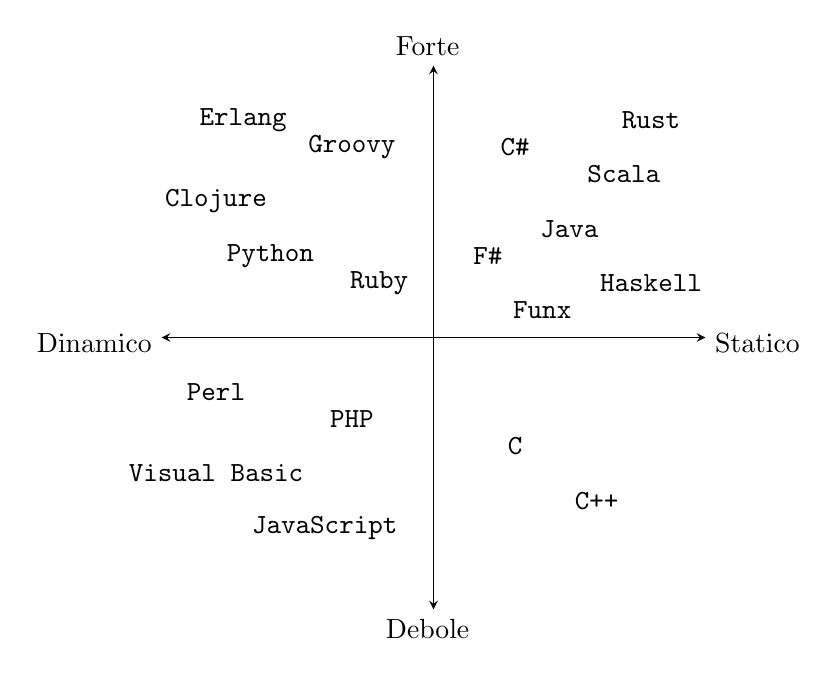
\begin{tikzpicture}
        \begin{axis}[
                % axis shenanigans
                width=0.7\textwidth, height=0.7\textwidth,
                xmin=-10, xmax=10,
                ymin=-10, ymax=10,
                xtick={-10},
                extra x ticks={10},
                ytick={-10},
                extra y ticks={10},
                % multiple labels for axes are actually tick labels
                xticklabels={Dinamico},
                extra x tick labels={Statico},
                yticklabels={Debole},
                extra y tick labels={Forte},
                % mess of a latex, with inconsistent package syntax
                tick style={draw=none},
                x tick label style={left},
                extra x tick style={xticklabel style={right}},
                y tick label style={below},
                extra y tick style={yticklabel style={above}},
                axis lines=middle,
                axis line style={stealth-stealth},
                clip=false
            ]
            % bleh
            \node at (axis cs:-8,-5) {\texttt{Visual Basic}};
            \node at (axis cs:-4,-7) {\texttt{JavaScript}};
            \node at (axis cs:-8,-2) {\texttt{Perl}};
            \node at (axis cs:-3,-3) {\texttt{PHP}};
            % meh
            \node at (axis cs:-7,8) {\texttt{Erlang}};
            \node at (axis cs:-8,5) {\texttt{Clojure}};
            \node at (axis cs:-3,7) {\texttt{Groovy}};
            \node at (axis cs:-6,3) {\texttt{Python}};
            \node at (axis cs:-2,2) {\texttt{Ruby}};
            % okay
            \node at (axis cs:3,-4) {\texttt{C}};
            \node at (axis cs:6,-6) {\texttt{C++}};
            % good
            \node at (axis cs:3,7) {\texttt{C\#}};
            \node at (axis cs:4,1) {\texttt{Funx}}; % bleh amongst the good
            \node at (axis cs:5,4) {\texttt{Java}};
            \node at (axis cs:2,3) {\texttt{F\#}};
            \node at (axis cs:7,6) {\texttt{Scala}};
            \node at (axis cs:8,2) {\texttt{Haskell}}; % hell yeah
            \node at (axis cs:8,8) {\texttt{Rust}}; % divine
        \end{axis}
    \end{tikzpicture}
    \caption{Alcuni linguaggi e loro sistemi di tipo}
    \label{fig:3-languages-type-systems}
    \vspace{8mm}
\end{figure}

\noindent Grazie ai tipi dinamici, linguaggi quali \texttt{Python} e \texttt{JavaScript} permettono
veloce prototipazione, flessibilità e codice più conciso, a discapito però di una più alta
probabilità di incontrare errori importanti a runtime, piuttosto che in fase di compilazione.


Al contrario, i tipi statici spesso migliorano naturalmente la mantenibilità di un progetto:
viene limitata la possibilità di scorciatoie nello sviluppo, ma si hanno maggiori garanzie di correttezza,
in quanto il compilatore può implementare ulteriori controlli e segnalare errori semantici più precisi già
prima dell'esecuzione del programma.

\noindent D'altro canto, l'obbligo di specificare i tipi di ogni variabile, oggetto, funzione e
parametro può risultare tedioso e talvolta ridondante; molti linguaggi moderni,
tra cui \texttt{Haskell} e \texttt{Rust}, ovviano magistralmente a quest'inconvenienza tramite
l'uso dell'inferenza di tipo.

\noindent Gli algoritmi di inferenza introducono numerosi benefici, in particolare:
\begin{itemize}
    \item la scrittura del codice è meno onerosa per lo sviluppatore a prescindere dal sistema di tipi utilizzato,
          e diviene quindi estremamente vantaggioso utilizzare tipi statici;
    \item le annotazioni ora opzionali possono essere aggiunte dal programmatore quando vi sono casi difficili
          da disambiguare automaticamente, oppure per migliorare la leggibilità del codice;
    \item gli strumenti di sviluppo per il linguaggio possono sfruttare informazioni fornite dal motore di inferenza
          per suggerire il tipo delle espressioni e arricchire i messaggi di errore e di warning.
\end{itemize}
\chapter{Java}
\label{chap:4-java}

Parallelamente alle prime fasi di sviluppo è stata svolta un'analisi di \texttt{Java}%
\footnote{OpenJDK (\url{https://openjdk.org})}
per valutare quali fossero le caratteristiche del linguaggio utili alla traduzione di codice \textbf{Funx}.

\noindent Questo capitolo riporta pertanto una breve panoramica delle principali funzionalità impiegate,
accompagnate da esempi di traduzione che illustrano alcuni dei risultati ottenibili con il compilatore
(si ricorda che altri esempi sono esibiti durante il Capitolo~\ref{chap:5-compiler}).

Le funzioni non dichiarate all'interno degli esempi stessi provengono dalla piccola libreria standard
(suddivisa in \texttt{FunxPrelude} e \texttt{JavaPrelude}, di cui la seconda include funzioni necessariamente definite in \texttt{Java}),
parzialmente presentata nella Tabella~\ref{tab:2-4-sugar} con gli operatori simbolici.

\section{Interfacce funzionali}
\label{sec:4-1-functional-interfaces}

Nel tradurre un linguaggio funzionale viene naturale pensare immediatamente alle \textit{interfacce funzionali} e \textit{lambda espressioni}
introdotte in \texttt{Java} 8%
\footnote{OpenJDK 8 (\url{https://openjdk.org/projects/jdk8})}
per rappresentare funzioni anonime: l'interfaccia generica \texttt{Function} è la più adatta a riprodurre
il comportamento dell'astrazione, come mostrato nei Codici~\ref{lst:4-1-function-funx}~e~\ref{lst:4-1-function-java}.

\vspace{4mm}
\begin{lstlisting}[caption={Semplice funzione in \textbf{Funx}}, style=funxCode, label={lst:4-1-function-funx}]
constant : a @-> b @-> a
constant x = \y @-> x
\end{lstlisting}
\vspace{4mm}
\begin{lstlisting}[caption={Corrispondente metodo in \texttt{Java}}, style=javaCode, label={lst:4-1-function-java}]
public static @<a, b@> Function@<a, Function@<b, a@>@> constant() {
    return (x @-> (y @-> x));
}
\end{lstlisting}
\vspace{4mm}

\noindent Dato il naturale \textit{currying} di oggetti \texttt{Function}, questo tipo di traduzione ha il vantaggio
di permettere l'applicazione parziale di funzioni (tramite una sequenza di \texttt{apply()} in numero minore rispetto al totale degli input),
ma il grande svantaggio della creazione di una nuova istanza della funzione per ogni chiamata.


Poiché \texttt{constant} ha tipo polimorfo (sezione~\ref{sec:4-3-generics}), il metodo utilizza parametri di tipo
e deve quindi necessariamente restituire un nuovo oggetto con ogni chiamata:
nonostante la performance delle traduzioni non sia un obiettivo primario del progetto, la versione attuale
del compilatore fa uso di alcune piccole ottimizzazioni nella trasposizione delle funzioni monomorfe,
approfondite nella sezione~\ref{sec:5-13-monomorphic-declarations}.

\newpage

\noindent In aggiunta alla classe \texttt{Function}, nella parte nativa (codice \texttt{Java}) della libreria standard
di \textbf{Funx} è definita un'ulteriore interfaccia funzionale per creare espressioni \texttt{let}:
in questo caso vi è un grande utilizzo di classi anonime, potenzialmente annidate,
rappresentanti le dichiarazioni locali e l'espressione principale (metodo \texttt{eval}).

\vspace{4mm}
\begin{lstlisting}[caption={Interfaccia funzionale per espressioni \texttt{let}}, style=javaCode, label={lst:4-1-let-interface-java}]
@FunctionalInterface
public interface Let@<T@> {
    T _eval();
}
\end{lstlisting}
\vspace{4mm}
\begin{lstlisting}[caption={Espressione \texttt{let} in \textbf{Funx}}, style=funxCode, label={lst:4-1-let-funx}]
hundredsSum : Int @-> Int @-> Int
hundredsSum = let
        on : (a @-> a @-> b) @-> (c @-> a) @-> c @-> c @-> b
        on op f x y = op (f x) (f y)
    in on add (multiply 100)
\end{lstlisting}
\vspace{4mm}
\begin{lstlisting}[caption={Corrispondente classe anonima in \texttt{Java}}, style=javaCode, label={lst:4-1-let-java}]
public static Function@<Long, Function@<Long, Long@>@> hundredsSum;

static {
    hundredsSum = (new Let@<@>() {
        private @<a, b, c@>
            Function@<
                    Function@<a, Function@<a, b@>@>,
                    Function@<Function@<c, a@>, Function@<c, Function@<c, b@>@>@>@>
                on() {
            return (op @-> (f @-> (x @-> (y @-> op.apply(f.apply(x)).apply(f.apply(y))))));
        }

        @Override
        public Function@<Long, Function@<Long, Long@>@> _eval() {
            return this.@<Long, Long, Long@>on().apply(add).apply(multiply.apply(100L));
        }
    })._eval();
}
\end{lstlisting}
\vspace{4mm}

\noindent Nei Codici~\ref{lst:4-1-let-funx}~e~\ref{lst:4-1-let-java} si può vedere che la funzione \texttt{hundredsSum}
è implementata attraverso la chiamata al metodo principale dell'interfaccia funzionale \texttt{Let},
realizzato internamente alla classe anonima con il supporto del metodo polimorfo \texttt{on}.

\noindent Inoltre, è immediatamente evidente come le traduzioni in \texttt{Java} siano progressivamente più complesse e meno leggibili
con l'introduzione di nuove funzionalità: l'esempio più eclatante è dato proprio dal tipo di ritorno del metodo locale \texttt{on},
divenuto di difficile comprensione rispetto alla sintassi molto concisa del linguaggio funzionale.

\newpage

\section{Operatore ternario}
\label{sec:4-2-ternary-operator}

Una delle peculiarità della traduzione da \textbf{Funx} a \texttt{Java} è l'uso dell'operatore ternario
(\texttt{condition ? thenBranch : elseBranch}) ogni qualvolta
siano presenti espressioni condizionali \texttt{if-then-else}.


I linguaggi funzionali sfruttano spesso una caratteristica (non menzionata nella sezione~\ref{sec:2-1-functional-languages})
che prende il nome di \textit{lazy evaluation} (valutazione pigra): fino a quando il risultato di un'espressione
non è richiesto per un successivo calcolo, questa non verrà completamente valutata.

\noindent Oltre ad offrire molteplici possibilità di ottimizzazione dal punto di vista del tempo di esecuzione,
tale comportamento è molto comodo nella scrittura di funzioni che per esempio potrebbero terminare
prima del previso o magari effettuare computazioni su strutture dati infinite.
I linguaggi che sono \textit{lazy evaluated} di default impegano nella maggior parte dei casi un \textit{garbage collector}
per liberare la memoria occupata dalle espressioni non valutate e non più rilevanti.


Il linguaggio \texttt{Java} non adotta la \textit{lazy evaluation} di default se non in casi particolari, tra cui
gli operatori booleani binari, il costrutto \texttt{if-then-else} (e corrispondente operatore ternario) e altre
funzionalità più avanzate tra cui gli \textit{stream} e le \textit{lambda espressioni} già viste.
Utilizzando quest'ultime si potrebbero ottenere risultati simili, in termini di valutazione pigra, a quelli di un linguaggio funzionale;
tuttavia, rendere \textbf{Funx} un linguaggio completamente pigro avrebbe comportato una traduzione indubbiamente ancora più complessa,
molteplici rischi di peggiorare le prestazioni dei programmi e un'implementazione del compilatore che va oltre lo scopo di questo progetto.


Nonostante ciò, la scelta di ridurre gli operatori booleani binari (\textit{and} e \textit{or}) ad espressioni con operatore ternario
è stata considerata quasi obbligatoria per conservarne la natura pigra: gli operatori ternari utilizzati a questo scopo
derivano direttamente dalla costruzione dell'\textbf{AST} (sezione~\ref{sec:5-6-ast-builder}), motivo per cui non vengono riconvertiti
in operatori nativi di \texttt{Java} in fase di traduzione.

\vspace{4mm}
\begin{lstlisting}[caption={If e operatori booleani in \textbf{Funx}}, style=funxCode, label={lst:4-2-ternary-funx}]
power : Int @-> Int @-> Int
power b e = if e == 0 then 1 else b * power b (e - 1) fi

xor : Bool @-> Bool @-> Bool
xor a b = (a || b) && !!(a && b)
\end{lstlisting}
\vspace{4mm}
\begin{lstlisting}[caption={Corrispondenti operatori ternari in \texttt{Java}}, style=javaCode, label={lst:4-2-ternary-java}]
public static Function@<Long, Function@<Long, Long@>@> power;

public static Function@<Boolean, Function@<Boolean, Boolean@>@> xor;

static {
    power = (b @-> (e @-> ((JavaPrelude.@<Long@>equalsEquals().apply(e).apply(0L))
        @? (1L)
        @: (multiply.apply(b)
            .apply(power.apply(b).apply(subtract.apply(e).apply(1L)))))));

    xor = (a @-> (b @->
        ((((a) @? (true) @: (b))) @? (not.apply(((a) @? (b) @: (false)))) @: (false))));
}
\end{lstlisting}


\newpage

\section{Tipi generici}
\label{sec:4-3-generics}

Il sistema di tipo di \textbf{Funx} necessita la traduzione di funzioni polimorfe,
e la soluzione più semplice e idiomatica in \texttt{Java} è l'utilizzo dei \textit{generics}:
tramite i parametri di tipo generici è possibile definire classi e metodi che agiscono su molteplici tipi di dati,
implementando comportamenti che possono essere condivisi dai diversi elementi del dominio di tipi delle funzioni rappresentate.


Nel contesto del \textit{sistema HM} di \textbf{Funx}, le variabili quantificate universalmente nei politipi
hanno una diretta corrispondenza con i parametri di tipo che possono essere dichiarati tra i modificatori di visibilità
e il tipo di ritorno di un metodo, il quale a sua volta combacia con la parte interna dello schema di tipo.


Nei Codici~\ref{lst:4-3-generics-funx}~e~\ref{lst:4-3-generics-java} si può notare come \texttt{Java} non sempre sia in grado
d'inferire i tipi desiderati per le funzioni polimorfe: queste devono infatti essere istanziate esplicitamente
usando la classe di appartenenza e le parentesi angolari (questa limitazione richiederà alcuni espedienti in casi limite
illustrati nelle sezioni~\ref{sec:5-14-polymorphic-functions-instantiation}~e~\ref{sec:5-15-wild-type-casting}).

\vspace{4mm}
\begin{lstlisting}[caption={Scrittura e utilizzo di funzioni polimorfe in \textbf{Funx}}, style=funxCode, label={lst:4-3-generics-funx}]
sumToN : Int @-> Int
sumToN = let
        ap : (a @-> b @-> c) @-> (a @-> b) @-> a @-> c
        ap op f x = op x (f x)
    in (flip divide 2) . ap multiply (add 1)
\end{lstlisting}
\vspace{4mm}
\begin{lstlisting}[caption={Corrispondenti proprietà e metodi \texttt{Java}}, style=javaCode, label={lst:4-3-generics-java}]
public static Function@<Long, Long@> sumToN;

static {
    sumToN = (new Let@<@>() {
        private @<a, b, c@>
            Function@<
                Function@<a, Function@<b, c@>@>,
                Function@<Function@<a, b@>, Function@<a, c@>@>@>
                    ap() {
            return (op @-> (f @-> (x @-> op.apply(x).apply(f.apply(x)))));
        }

        @Override
        public Function@<Long, Long@> _eval() {
            return FunxPrelude.@<Long, Long, Long@>compose()
                .apply(FunxPrelude.@<Long, Long, Long@>flip().apply(divide).apply(2L))
                .apply(this.@<Long, Long, Long@>ap().apply(multiply).apply(add.apply(1L)));
        }
    })._eval();
}  
\end{lstlisting}

\chapter{\localized{Compilatore}{Compiler}}
\label{chap:5-compiler}

Il software sviluppato per il progetto è stato sviluppato mantenendo il codice sul repository \texttt{GitHub} \textbf{Funx-jt}%
\footnote{massimopavoni/Funx-jt (\url{https://github.com/massimopavoni/Funx-jt})},
nel cui nome \textit{"jt"} è l'acronimo per \textit{"Java Transpiler"}.

\noindent La prima release stabile è disponibile sul repository (\texttt{Funx-jt-0.1.0})
con una \textit{Command Line Interface} per traduzione ed esecuzione di programmi \textbf{Funx};
è stato utilizzato \texttt{Gradle}%
\footnote{Gradle Build Tool (\url{https://gradle.org})}
per la compilazione e la gestione delle dipendenze,
assieme alla più recente versione \textit{Long Term Support (LTS)} di \texttt{Java}, OpenJDK 21%
\footnote{OpenJDK 21 (\url{https://openjdk.org/projects/jdk/21})}.

Nel corso di questo capitolo si discuteranno le fasi di compilazione e la struttura del software,
analizzando nel dettaglio le parti più importanti.

\begin{figure}
    \vspace{4mm}
    \begin{minipage}{0.85\textwidth}
        \includegraphics[width=\linewidth]{funx-jt-h.png}
        \vspace{2mm}
    \end{minipage}
    \begin{minipage}{0.85\textwidth}
        \includegraphics[width=\linewidth]{funx-jt-t-h.png}
        \vspace{2mm}
    \end{minipage}
    \begin{minipage}{0.85\textwidth}
        \includegraphics[width=\linewidth]{funx-jt-r-h.png}
    \end{minipage}
    \caption{Possibili comandi e opzioni della \textit{CLI}}
    \label{fig:5-compiler-cli}
\end{figure}

\newpage

\section{ANTLR}
\label{sec:5-1-antlr}

Al fine di semplificare lo sviluppo di \textit{lexer} e \textit{parser} per il linguaggio funzionale ideato
è stato scelto il generatore di \textit{parser} chiamato \texttt{ANTLR}%
\footnote{ANother Tool for Language Recognition;
    \citetitle{Parr-1995-ANTLRGenerator} \cite{Parr-1995-ANTLRGenerator},
    \citetitle{Parr-2013-DefinitiveANTLR} \cite{Parr-2013-DefinitiveANTLR}
    and ANTLRv4 (\url{https://www.antlr.org})}.

\noindent Grazie a tale strumento il processo iterativo di creazione della grammatica di \textbf{Funx}
è stato notevolmente semplificato e accelerato, in quanto \texttt{ANTLR} mette a disposizione del programmatore
un linguaggio per definire uno o più file di specifica per lessico e sintassi
(directory \texttt{Funx-jt/src/main/antlr} nel repository): questi vengono poi processati
per generare il codice sorgente del \textit{lexer} e del \textit{parser}.

\subsection{Analisi lessicale}
\label{sec:5-2-lexical-analysis}

Data la probabile complessità delle regole della grammatica di \textbf{Funx}, fin dall'inizio la definizione dei \textit{token} (lessemi)
del linguaggio è stata separata dalla specifica del \textit{parser}.

\noindent Il file \texttt{FunxLexer.g4} descrive i lessemi dividendoli nelle seguenti cateogorie:
\begin{enumerate}
    \item \textit{whitespace}: caratteri di spaziatura e tabulazione;
    \item \textit{comments}: commenti di linea e blocco;
    \item \textit{keywords}: parole chiave del linguaggio;
    \item \textit{Java keywords}: parole chiave del linguaggio Java, da evitare;
    \item \textit{types}: tipi di dato (funzioni di tipo con arità 0);
    \item \textit{literals}: costanti booleane e numeriche;
    \item \textit{variables}: identificatori per variabili di tipo o nomi di funzioni;
    \item \textit{module}: identificatori il modulo;
    \item vari operatori simbolici per:
          \begin{itemize}
              \item \textit{bool}: valori booleani;
              \item \textit{comparison}: confronti tra numeri;
              \item \textit{arithmetic}: operazioni aritmetiche;
              \item \textit{other symbols}: simboli della sintassi (come \texttt{->}) e varie funzioni di libreria;
              \item \textit{delimiters}: parentesi tonde, quadre e graffe.
          \end{itemize}
\end{enumerate}

\noindent Le categorie 1 e 2 contengono token da scartare, tranne \texttt{NEWLINE}, mentre la categoria 4 è utile
qualora eventualmente si permetta allo sviluppatore di utilizzare tali parole chiave riservate,
effettuando una rinomina automatica; le categorie 7 e 8 devono necessariamente apparire dopo le categorie 3 e 4,
poiché tra \textit{keyword} e identificatori di ogni genere le prime devono avere la precedenza
(la posizione della categoria 5 tiene conto di una possibile futura estensione per consentire la creazione di nuovi tipi).

Oltre alle categorie illustrate, in testa al file sono presenti dei cosiddetti \textit{fragment} (frammenti)
che semplificano le espressioni regolari dei \textit{token} e complessivamente aumentano la leggibilità della specifica.

\newpage

\begin{lstlisting}[caption={Alcune \textit{token} del \textit{lexer}}, style=antlrCode, label={lst:5-lexer}]
lexer grammar FunxLexer;

// Fragments
fragment LALPHA: [a-z];
fragment UALPHA: [A-Z];
fragment ALPHA: LALPHA | UALPHA;
fragment ALPHA_: ALPHA | UnderScore;

fragment DIGIT: [0-9];
fragment DECIMAL: DIGIT+;

// Whitespace
NEWLINE: '\r'? '\n' | '\r';

TAB: [\t]+ @-> skip;
WS: [\u0020\u00a0\u1680\u2000\u200a\u202f\u205f\u3000]+ @-> skip;

// Comments
CloseMultiComment: '\./';
OpenMultiComment: '/\.';
SingleComment: '//';

COMMENT: SingleComment ~[\r\n]* @-> skip;
MULTICOMMENT: OpenMultiComment .*? CloseMultiComment @-> skip;

// Keywords
ELSE: 'else';
FI: 'fi';
IF: 'if';
IN: 'in';
LET: 'let';

// Java keywords
RESERVED_JAVA_KEYWORD: 'abstract' | 'assert' | 'boolean' | 'break' | 'byte' | [\.\.\.];

// Types
TYPE: BOOLTYPE | INTTYPE;
BOOLTYPE: 'Bool';

// Literals
INT: DECIMAL | OpenParen '\-' DECIMAL CloseParen;

// Variables
VARID: LALPHA (ALPHA_ | DIGIT)*;

// Module
MODULEID: UALPHA (ALPHA_ | DIGIT)*;

// Bool
And: '&&';
Not: '!!';

// Comparison
EqualsEquals: '\=\=';
NotEquals: '!\=';

// Arithmetic
Add: '\+';

// Other symbols
UnderScore: '_';
Arrow: '\-\>';

// Delimiters
OpenParen: '\(';
CloseParen: '\)';
\end{lstlisting}

\subsection{Analisi sintattica}
\label{sec:5-3-syntactic-analysis}

Il file \texttt{FunxParser.g4} contiene le regole concrete della grammatica di \textbf{Funx}:
nonostante la somiglianza con le grammatiche delle Figure~\ref{fig:2-3-funx-syntax}~e~\ref{fig:3-3-system-hm},
è evidente che queste non collimino esattamente a causa di zucchero sintattico e requisiti di \texttt{ANTLR}.

\noindent Lo strumento utilizzato, infatti, è un generatore di \textit{parser} di tipo \textit{top-down}
per grammatiche \textit{LL}, le quali in generale non supportano regole ricorsive a sinistra.

\noindent Essendo tali regole spesso comuni nella definizione di qualsiasi linguaggio di programmazione, \textbf{Funx} incluso,
\texttt{ANTLRv4} offre un diverso tipo di parsing, detto \textit{Adaptive LL(*)} \cite{Parr-2011-FoundationANTLR,Parr-2014-AdaptiveLL}:
quest'ultimo è in grado di riscrivere automaticamente le grammatiche, eliminando la ricorsione a sinistra diretta (e.g. linee 36 e 38-43),
così da non incorrere in regole ambigue che potrebbero causare \textit{backtracking} e conseguente \textit{overhead}.

\noindent Il Codice~\ref{lst:5-3-parser-antlr} riporta integralmente le regole concrete della sintassi di \textbf{Funx}, tra cui:
\begin{itemize}
    \item \textit{module}: nome del modulo, funzione \texttt{main} opzionale e dichiarazioni globali;
    \item \textit{main}: funzione \texttt{main}, diversa dalle dichiarazioni classiche per l'assenza di schema di tipo e parametri lambda;
    \item \textit{declaration}: funzione con nome, tipo e parametri (e opzionalmente \texttt{with} per funzioni locali);
    \item \textit{typeElems}: tipo di una funzione, definito ricorsivamente secondo la grammatica del sistema di tipo di \textbf{Funx};
    \item \textit{statement}: per evitare ricorsione a sinistra indiretta, la separazione tra \textit{statement} ed \textit{expression}
          forza l'uso di parentesi nei casi in cui lambda astrazioni, let e if siano usati all'interno di un'espressione;
    \item \textit{expression}: racchiude l'applicazione funzionale, tutte le regole relative agli operatori simbolici,
          specificandone la priorità implicita (Tabella~\ref{tab:2-4-sugar}), e le espressioni primarie
          (costanti, variabili e parentesi per controllare la precedenza);
    \item \textit{lambda, let, if}: corrispondenti alle produzioni per astrazione, let e if della grammatica formale.
\end{itemize}

\newpage

\begin{lstlisting}[caption={Grammatica per il \textit{parser}}, style=antlrCode, label={lst:5-3-parser-antlr}]
parser grammar FunxParser;
options { tokenVocab = FunxLexer; }

// Module
module: (MODULE MODULEID (Dot MODULEID)* NEWLINE+)?
    (main NEWLINE+)? declarations EOF;

declarations: declaration (NEWLINE declaration?)*;

main: id = MAIN Equals statement with?;

// Declaration
declaration: (declarationScheme NEWLINE)?
    id = VARID lambdaParams? Equals statement with?;

declarationScheme: id = VARID Colon typeElems;

with: NEWLINE WITH localDeclarations OUT;

localDeclarations: NEWLINE declarations NEWLINE;

// Type
typeElems: OpenParen typeElems CloseParen %# parenType%
    | VARID %# typeVar%
    | TYPE %# namedType%
    | <assoc = right> typeElems Arrow typeElems %# arrowType%;

// Statement
statement: expression %# expressionStatement%
    | lambda %# lambdaStatement%
    | let %# letStatement%
    | ifS %# ifStatement%;

// Expression
expression: primary %# primExpression%
    | expression expression %# appExpression%
    | <assoc = right> expression bop = Dot expression %# composeExpression%
    | expression bop = (Divide | Modulo | Multiply) expression %# divModMultExpression%
    | expression bop = (Add | Subtract) expression %# addSubExpression%
    | expression
        bop = (GreaterThan | GreaterThanEquals | LessThan | LessThanEquals)
        expression %# compExpression%
    | expression bop = (EqualsEquals | NotEquals) expression %# eqExpression%
    | uop = Not expression %# notExpression%
    | <assoc = right> expression bop = And expression %# andExpression%
    | <assoc = right> expression bop = Or expression %# orExpression%
    | <assoc = right> expression bop = Dollar expression %# rightAppExpression%;

primary: OpenParen statement CloseParen %# parenPrimary%
    | constant %# constPrimary% | VARID %# varPrimary%;

// Lambda
lambda: Backslash lambdaParams? Arrow statement;

lambdaParams: VARID+;

// Let
let: LET localDeclarations IN statement;

// If
ifS: IF statement THEN statement ELSE statement FI;

// Constant
constant: BOOL | numConstant;

numConstant: INT;    
\end{lstlisting}

\section{Albero sintattico astratto}
\label{sec:5-4-abstract-syntax-tree}

\subsection{Gerarchia delle classi}
\label{sec:5-5-class-hierarchy}

Il primo passo per la costruzione di un \textbf{AST} per la sintassi di \textbf{Funx} è la definizione
di una gerarchia di classi \texttt{Java} che rappresentano i nodi dell'albero
(package \texttt{com.github.massimopavoni.funx.jt.ast.node}).


La classe astratta \texttt{ASTNode} è la radice dell'ordinamento poiché sarà usata per gli oggetti creati
a partire dal \textit{CST}: contiene la proprietà \texttt{inputPosition} per facilitare la segnalazione di errori
e vincola le classi figlie all'implementazione del metodo astratto \texttt{accept} per visitare i nodi.

\noindent Un'altra classe astratta, derivata dalla precedente, è \texttt{Expression}, la quale identifica
un'espressione ed è dotata di alcuni campi e metodi utili all'inferenza di tipo.


Ogni altra sottoclasse (ad eccezione di \texttt{Declarations}, utilizzata per dichiarazioni globali e locali)
è una trascrizione in \texttt{Java} delle produzioni della grammatica formale:
\begin{itemize}
    \item \texttt{Module}: modulo del programma;
    \item \texttt{Declaration}: dichiarazione di funzione;
    \item \texttt{Constant}: termini costanti;
    \item \texttt{Variable}: simboli per variabili;
    \item \texttt{Application}: applicazione di funzione;
    \item \texttt{Lambda}: astrazione per le funzioni anonime;
    \item \texttt{Let}: contenitore di dichiarazioni locali;
    \item \texttt{If}: costrutto condizionale.
\end{itemize}

\newpage

\begin{figure}
    \begin{tikzpicture}
        \umlsimpleclass[type=abstract]{ASTNode}
        \umlsimpleclass[x=4,type=interface]{Inferable}
        \umlsimpleclass[x=-4,y=-2]{Module}
        \umlsimpleclass[y=-2]{Declarations}
        \umlsimpleclass[x=4,y=-2,type=abstract]{Expression}
        \umlsimpleclass[x=-2,y=-3.5]{Constant}
        \umlsimpleclass[x=-2,y=-5]{Variable}
        \umlsimpleclass[x=-2,y=-6.5]{Application}
        \umlsimpleclass[x=-2,y=-8]{Lambda}
        \umlsimpleclass[x=-2,y=-9.5]{Let}
        \umlsimpleclass[x=-2,y=-11]{If}
        \umlinherit[geometry=|-]{Module}{ASTNode}
        \umlinherit{Declarations}{ASTNode}
        \umlinherit[geometry=-|-]{Expression}{ASTNode}
        \umlimpl{Expression}{Inferable}
        \umlinherit[geometry=-|,anchor2=-160]{Constant}{Expression}
        \umlinherit[geometry=-|,anchor2=-149]{Variable}{Expression}
        \umlinherit[geometry=-|,anchor2=-117]{Application}{Expression}
        \umlinherit[geometry=-|,anchor2=-63]{Lambda}{Expression}
        \umlinherit[geometry=-|,anchor2=-31]{Let}{Expression}
        \umlinherit[geometry=-|,anchor2=-20]{If}{Expression}
    \end{tikzpicture}
    \caption{Diagramma semplificato delle classi dell'\textbf{AST}}
    \label{fig:5-ast-classes}
    \vspace{4mm}
\end{figure}

\begin{lstlisting}[caption={Esempio di classe della gerarchia}, style=javaCode, label={lst:5-class-example-java}]
public static final class Lambda extends Expression {
    public final String paramId;

    public final Expression expression;

    public Lambda(InputPosition inputPosition, String paramId, ASTNode expression) {
        super(inputPosition); // ASTNode constructor
        this.paramId = paramId;
        this.expression = (Expression) expression;
    }

    @Override // from Inferable interface
    public Utils.Tuple<Substitution, Type> infer(Context ctx) { ... }

    @Override // from Expression abstract class
    protected void propagateSubstitution(Substitution substitution) { ... }

    @Override // from ASTNode abstract class
    public @<T@> T accept(ASTVisitor<? extends T> visitor) {
        return visitor.visitLambda(this);
    }
}
\end{lstlisting}



\subsection{AST builder}
\label{sec:5-6-ast-builder}



\section{Motore inferenziale}
\label{sec:5-7-inference-engine}

I sistemi di tipo e l'inferenza descritti nel Capitolo~\ref{chap:3-inference} costituiscono una parte imprescindibile del software,
data l'incapacità di simulare il polimorfismo parametrico del \textit{sistema HM} lasciando al compilatore \texttt{Java}
il compito di inferire e controllare i tipi dei metodi (o classi) generici.
In tal caso, infatti, la compilazione fallirebbe a causa di tipi "troppo generici" e \textit{type casting} non permesso
in maniera implicita (e.g. non si è in grado di conciliare ad esempio un tipo generico con una lambda espressione).

\begin{figure}
    \vspace{4mm}
    \includegraphics[width=\textwidth]{5-7-impossible-java.png}
    \caption{Esempio di errore in \texttt{Java} dovuto a tipi generici}
    \label{fig:5-7-impossible-java}
    \vspace{4mm}
\end{figure}

\noindent La linea di codice citata in Figura~\ref{fig:5-7-impossible-java} non è intrinsecamente errata,
ma non può essere compilata in mancanza di informazioni riguardanti il parametro di tipo generico della funzione \texttt{id}
(con tipo di ritorno \texttt{Function<T, T>}): il problema da risolvere è quindi conoscere il tipo dell'espressione
in input alla prima chiamata al metodo \texttt{apply}.


Il motore inferenziale è la parte del compilatore che si occupa di stabilire i tipi delle espressioni seguendo le regole
di inferenza e i passi dell'\textit{algoritmo $\mathcal{W}$}%
\footnote{\citetitle{Grabmuller-2006-AlgorithmW} \cite{Grabmuller-2006-AlgorithmW}}
descritti nella sezione~\ref{sec:3-4-hm-type-inference}; la fase di inferenza avviene subito dopo il parsing
e la costruzione dell'\textbf{AST} e precede la generazione del codice \texttt{Java}.

\subsection{Sistema HM}
\label{sec:5-8-system-hm}


\newpage

\subsection{Inferenza su espressioni}
\label{sec:5-9-expression-inference}


\section{Traduzione in Java}
\label{sec:5-10-java-translation}

La sottoclasse più importante di \texttt{ASTVisitor} è \texttt{JavaTranspiler}, il \textit{visitor} che si occupa
dell'ultimo stadio di compilazione, la traduzione dell'\textbf{AST} in codice \texttt{Java}:
come per \texttt{GraphvizBuilder}, la classe compone una stringa
che rappresenta il programma \texttt{Java} corrispondente al codice \textbf{Funx} sorgente.


Avendo già illustrato alcuni esempi di traduzione nel Capitolo~\ref{chap:4-java}, in questa sezione si
discuteranno le scelte e i compromessi nel processo di traduzione, e il modo in cui le limitazioni
di \texttt{Java} possano essere talvolta aggirate "piegando" le regole.

\subsection{Membri statici}
\label{sec:5-11-static-members}

Il paradigma dichiarativo dei linguaggi funzionali è ben diverso dalla programmazione ad oggetti di molti altri linguaggi rinomati,
motivo per cui la scelta di tradurre ogni programma \textbf{Funx} in un'unica classe statica è vista come semplice soluzione
per evitare complicanze e \textit{overhead} per la creazione di oggetti in aggiunta alle \texttt{Function}.


Ogni funzione definita diviene perciò una proprietà statica della classe in caso di monotipi (sezione~\ref{sec:5-13-monomorphic-declarations})
o un metodo statico con parametri di tipo in caso di politipi (sezione~\ref{sec:5-14-polymorphic-functions-instantiation}).
Fanno eccezione le funzioni appartenenti a espressioni \texttt{let} annidate: essendo classi anonime, queste creano
un unico oggetto con proprietà e metodi privati (accessibili solamente al metodo pubblico \texttt{eval} della classe \texttt{Let}).

\noindent La traduzione inizia con \textit{import} statici per la libreria standard e un costruttore privato.

\vspace{4mm}
\begin{lstlisting}[caption={Prime aggiunte alla stringa \texttt{Java}}, style=javaCode, label={lst:5-11-first-append-java}]
// append package, imports, class declaration and constructor
builder.append(module.packageName.isEmpty()
        @? ""
        @: String.format("package %s;%n", module.packageName.toLowerCase()))
    .append("\n\nimport ").append(Function.class.getName())
    .append(";\n\nimport ").append(JavaPrelude.class.getName())
    .append(";\n\nimport ").append(FunxPrelude.class.getName())
    .append(";\n\nimport static ").append(JavaPrelude.class.getName())
    .append(".*;\nimport static ").append(FunxPrelude.class.getName())
    .append(".*;\n\npublic class ").append(module.name).append(" {\n")
    .append("private ").append(module.name)
    .append("() {\n// private constructor to prevent instantiation\n}\n\n");
\end{lstlisting}
\vspace{4mm}
\begin{lstlisting}[caption={Corrispondente codice \texttt{Java} generato}, style=javaCode, label={lst:5-11-class-start-java}]
import java.util.function.Function;

import com.github.massimopavoni.funx.lib.JavaPrelude;

import com.github.massimopavoni.funx.lib.FunxPrelude;

import static com.github.massimopavoni.funx.lib.JavaPrelude.*;
import static com.github.massimopavoni.funx.lib.FunxPrelude.*;

public class Chapter5Header {
    private Chapter5Header() {
        // private constructor to prevent instantiation
    }

    // ...
}
\end{lstlisting}

\newpage

\subsection{Lista dei contesti}
\label{sec:5-12-scope-stack}

\subsection{Dichiarazioni monomorfe}
\label{sec:5-13-monomorphic-declarations}

La possibilità in \textbf{Funx} di utilizzare funzioni ricorsive (e/o mutuamente ricorsive)
e la volontà di evitare la traduzione in metodi quando possibile sono in conflitto
a causa di \textit{Illegal Self Reference} e \textit{Illegal Forward Reference}:
tali errori si presentano durante la compilazione del codice \texttt{Java}
qualora i campi statici che identificano funzioni monomorfe vengano dichiarati e inizializzati
nello stesso \textit{statement} (stessa linea).


La dichiarazione delle proprietà deve avvenire prima dell'inizializzazione di altre variabili che ne fanno uso;
si potrebbe effettuare un'analisi iniziale dell'\textbf{AST} per identificare le dipendenze tra le funzioni
(approccio di ordinamento topologico estremamente utile anche per l'inferenza), ma la soluzione adottata
è di più semplice implementazione.


Come si può notare nel Codice~\ref{lst:5-13-monomorphic-java} e in alcuni esempi già presentati in precedenza,
si effettua la dichiarazione di ogni campo, pubblico e statico per le dichiarazioni globali, privato per quelle locali,
e solo successivamente si inizializzano rispettivamente con blocco statico e metodo \texttt{eval}.

\vspace{4mm}
\begin{lstlisting}[caption={Esempio di traduzione per funzioni monomorfe}, style=javaCode, label={lst:5-13-monomorphic-java}]
public class Chapter5Monomorphic {
    private Chapter5Monomorphic() {
        // private constructor to prevent instantiation
    }
    
    public static void main(String[] args) {
        System.out.println(add.apply(add.apply(fun1).apply(fun2)).apply(letFun));
    }
    
    public static Long fun1;    
    public static Long fun2;    
    public static Long letFun;
    
    static {
        fun1 = 1L;    
        fun2 = 2L;    
        letFun =
            (new Let@<@>() {
                private Long a;    
                private Long b;
    
                @Override
                public Long _eval() {
                    a = 3L;
                    b = 4L;
                    return add.apply(a).apply(b);
                }
            })._eval();
    }
}
\end{lstlisting}

\newpage

\noindent Poiché potrebbero essere presenti diversi \texttt{let} annidati, è necessario tenere traccia delle espressioni
corpo delle dichiarazioni monomorfe in modo da poterle inizializzare al momento corretto, dopo aver tradotto ulteriori classi interne.

\noindent La procedura di traduzione di dichiarazioni monomorfe si compone delle seguenti fasi:
\begin{itemize}
    \item definizione di uno \textit{stack} contenente mappe tra nomi delle dichiarazioni e nodi espressione corrispondenti;
    \item inserimento di una nuova mappa per il livello corrente di annidamento (modulo o espressione \texttt{let});
    \item dichiarazione delle variabili e aggiunta delle espressioni monomorfe
          alla mappa corrente (potrebbero essere aggiunti nuovi livelli prima di poterne "riempire" uno);
    \item creazione del blocco statico (o metodo \texttt{eval} per le espressioni \texttt{let}) con l'inizializzazione
          delle funzioni monomorfe: in questa fase finale torna utile la versatilità del \textit{visitor pattern} per posticipare
          la traduzione delle espressioni.
\end{itemize}

\vspace{4mm}
\begin{lstlisting}[caption={Traduzione di funzioni monomorfe in \texttt{let}}, style=javaCode, label={lst:5-13-monomorphic-translation-java}]
private final Deque<Map<String, Expression>>
    monomorphicDeclarationsQueue = new ArrayDeque<>();

@Override
public Void visitLet(Expression.Let let) {
    currentLevel++;
    // ...
    // use a new anonymous class for the let expression
    // and push a new monomorphic let declarations map
    builder.append("(new ")
            .append(JavaPrelude.Let.class.getSimpleName()).append("<>() {\n");
    monomorphicDeclarationsQueue.push(new LinkedHashMap<>());
    visit(let.localDeclarations);
    builder.append("""
                    @Override
                    public\s""")
            .append(typeStringOf(let.expression.type()))
            .append("\n_eval() {\n");
    // if there are any monomorphic declarations, initialize them in the _eval method,
    // then pop the map either way
    if (!monomorphicDeclarationsQueue.getFirst().isEmpty())
        monomorphicDeclarationsQueue.getFirst().forEach((id, expression) @-> {
            builder.append(id).append(" = ");
            visit(expression); // deferred expression visit
            appendSemiColon();
            appendNewline();
        });
    monomorphicDeclarationsQueue.pop();
    // ...
    currentLevel--;
    return null;
}
\end{lstlisting}

\newpage

\begin{lstlisting}[caption={Metodo \texttt{visit} per le dichiarazioni}, style=javaCode, label={lst:5-13-visit-declaration-java}]
@Override
public Void visitDeclaration(Declaration declaration) {
    // top level declarations should be static and public,
    // while let local declarations should be private to the anonymous class
    builder.append(currentLevel == 0 @? "public static " @: "private ");
    String scheme = schemeStringOf(declaration.scheme());
    if (declaration.scheme().variables.isEmpty()) {
        // defer initialization of monomorphic declarations
        builder.append(scheme).append(" ").append(declaration.id);
        appendSemiColon();
        monomorphicDeclarationsQueue
            .getFirst().put(declaration.id, declaration.expression);
    } else {
        // initialize polymorphic declarations immediately (as methods with generics)
        builder.append(scheme)
                .append(" ").append(declaration.id).append("() {\nreturn ");
        visit(declaration.expression);
        appendSemiColon();
        appendCloseBrace();
    }
    appendNewline();
    return null;
}
\end{lstlisting}

\subsection{Instanziazione di funzioni polimorfe}
\label{sec:5-14-polymorphic-functions-instantiation}

\subsection{Type casting "selvaggio"}
\label{sec:5-15-wild-type-casting}

\chapter{\localized{Conclusioni}{Conclusions}}
\label{chap:6-conclusions}

All'epilogo del lavoro di tesi, è possibile affermare che il progetto è stato portato a termine con un più che discreto successo:
il linguaggio funzionle \textbf{Funx} è molto semplice ma può essere esteso per aumentarne l'espressività,
mentre il compilatore offre spazio per miglioramenti e ottimizzazioni.


Contemporaneamente, come ogni software, il risultato è lontano dall'essere perfetto,
e durante le fasi finali di sviluppo e di scrittura di questo documento sono emerse criticità e \textit{bug}
nel traduttore che ne inficiano affidabilità ed efficienza in alcuni rari casi, non scoperti in precedenza.


In questo breve capitolo verranno confrontati i risultati con gli obiettivi prefissati,
suggerite possibili estensioni per il linguagio e accennato un uso didattico.

\section{Obiettivi}
\label{sec:6-1-objectives}

Relativamente all'obiettivo di sviluppo del compilatore, l'approccio costruttivo della stringa \texttt{Java}
costituisce senz'altro una traduzione molto semplice e non eccessivamente intricata:
si è stati in grado di utilizzare le \textit{feature} menzionate nel Capitolo~\ref{chap:4-java} in modo
appropriato e in accordo con la specifica del piccolo linguaggio funzionale.


Le soluzioni ai problemi di \textit{parsing}, inferenza e generazione del codice si sono rivelate abbastanza
agili e corrette da favorire tempi di compilazione ed esecuzione accettabili, ma ovviamente non sufficienti
per giustificare la preferenza di \textbf{Funx} rispetto ad altri linguaggi maturi.
D'altro canto, il progetto non ha mai avuto simili pretese, e da subito è stato chiaro che la scelta della \texttt{JVM}
come piattaforma di destinazione avrebbe limitato le prestazioni dei programmi.


Per quanto il linguaggio permetta solamente di definire semplici funzioni usando numeri interi e costanti booleane,
le minime funzionalità di cui è dotato soddisfano i requisiti prestabiliti, inclusa la possibilità di ricorsione. 

\newpage

\section{Estensioni del linguaggio}
\label{sec:6-2-language-extensions}

Nel caso in cui si volesse continuare a sviluppare \textbf{Funx} e il compilatore annesso,
quelle che seguono sono alcune estensioni utili ad incrementarne notevolemente l'espressività:
\begin{itemize}
    \item \textbf{tuple}: nuovo tipo analogo alle tuple di \texttt{Haskell}, da ideare anche all'interno di \texttt{Java}
          stesso data la mancanza di supporto;
    \item \textbf{liste}: implementazione della corrispondenza tra le liste di \texttt{Java} e un nuovo tipo in \textbf{Funx},
          con il vantaggio di poter utilizzare alcune funzioni native;
    \item \textbf{stringhe}: la gestione di dati testuali si rivela essere potenzialmente tra le più complicate a seconda
          della traduzione dei singoli caratteri (utilizzare le liste in \texttt{Java} si rivelerebbe inefficiente);
    \item \textbf{switch-case}: aggiunta di una struttura di controllo più versatile rispetto all'attuale \texttt{if-else},
          affine alle \textit{switch expression} di \texttt{Java} e i \textit{case-of} di \texttt{Haskell};
    \item \textbf{tipi custom}: l'introduzione di tipi definiti dall'utente è un'altra espansione difficile da trattare,
          poiché la \textit{feature} di \texttt{Java} più idonea è l'uso delle classi, da generare sempre automaticamente;
    \item \textbf{suite di test}: con l'ampliamento del linguaggio, è indispensabile preparare una collezione di test
          per la verifica della correttezza del compilatore.
\end{itemize}

\section{Scopo educativo}
\label{sec:6-3-educational-purpose}

L'adozione di un linguaggio simile a \textbf{Funx} a scopo educativo offrirebbe opportunità significative
per arricchire l'insegnamento della programmazione, soprattutto dove \texttt{Java} e altri linguaggi
orientati agli oggetti dominano i curriculum: in ambito scolastico e accedemico si tende spesso a concentrarsi
molto sulla programmazione imperativa anche nelle fasi più avanzate dei corsi,
lasciando agli studenti l'approfondimento di altri paradigmi introdotti con minore importanza.

Alcuni concetti fondamentali di ogni linguaggio sono tuttavia più facilmente compresi attraverso la programmazione funzionale,
e l'uso di \textbf{Funx}, con una traduzione diretta in un linguaggio più familiare, sarebbe forse un modo per addolcire
la transizione ad un paradigma al quale la maggior parte degli studenti non è abituata.

\cleardoublepage
\phantomsection
\printbibliography[heading=bibintoc]

% \cleardoublepage
% \phantomsection
% \printindex

\chapter*{\localized{Ringraziamenti}{Special thanks}}
\label{chap:8-thanks}

Grazie al Prof. Luca Padovani per avermi fatto scoprire i linguaggi funzionali. \\
Grazie a tutti i professori che insegnando con passione hanno stimolato la mia curiosità. \\
\\
Grazie a tutti i colleghi studenti, passati e presenti. \\
Grazie ad Andrea, Nicola, Matteo e Thomas. \\
Grazie a Eduardo, Lorenzo e Marco. \\
Grazie davvero a Riccardo. \\
\\
\\
Grazie alla mia famiglia, papà, mamma e Davide. \\
Grazie a nonno, nonna, nonno e nonna, grazie ai cugini, grazie agli zii e alle zie. \\
\\
\\
Grazie ai miei amici, lontani e vicini. \\
Grazie ad Alessandro, Costanza, Matteo, Tiffany, Giuseppe e Giacomo. \\
Grazie a Gaetano, Matteo, Alberto, Endri e Stefano. \\
\\
Grazie di cuore a Luca, Tommaso, Antonio, Luca, Nicola e Began. \\
\\
\\
Grazie di tutto ad Anaya.
\\
\\
\\
\\
Mille grazie vanno a ciascuno di voi ché avete formato la mia persona e mi avete fatto compagnia
negli ultimi anni, e ad un'infinità di altre persone che sono state importanti in un modo o nell'altro.

\end{document}